%
% PKUMpLtX --- A LaTeX document class for 'Modern Physics Laboratory' in PKU based on `revtex4-2`
%
% Please read `README.md' and the template file before using
% 需要确保 font 选项指定的字体已安装! 具体参见 `README.md' 的说明.
\documentclass[font=default]{mpltx}

% 以下至 \begin{document} 都仅是本文件为了方便额外定义的命令, 写报告时不需要.
\hypersetup{colorlinks=true}% 超链接带颜色
\usepackage{xcolor}
\newcommand{\note}[1]{{\color{gray}#1}}
\NewDocumentCommand{\pkg}{s o m}{%
    \IfBooleanF{#1}{%
        \IfNoValueTF{#2}%
            {\href{https://www.ctan.org/pkg/#3}}%
            {\href{https://www.ctan.org/pkg/#2}}%
    }%
    {\textsf{#3}}%
}
\newcommand*\cs[1]{\texttt{\textbackslash #1}}
\newcommand*\env[1]{\textit{\texttt{#1}}}
\newcommand*\code[1]{\texttt{#1}}
\newcommand*\file[1]{\textbf{\texttt{#1}}}
\makeatletter
\newcommand\releasedate{%
    \href{https://github.com/CastleStar14654/PKUMpLtX/releases/tag/\mpltx@fileversion}%
        {\mpltx@filedate, \mpltx@fileversion}}
\makeatother
% 以上是本文件为了方便额外定义的命令, 写报告时不需要.

\begin{document}

\title{晶体的电光效应} % 切合报告内容, 简短明确, 可以不同于讲义
\author{李钰欣} % 这里 \emailphone 一定要紧跟在 \author 后方
\emailphone{2300011368@stu.pku.edu.cn}{(86)15816647600}
% 如果改用 \email 则仅需要邮箱参数
\affiliation{北京大学物理学院\quad 学号: 2300011368}
% % 可以使用 \zhdate 自动生成中文日期, 如
% \date{\zhdate{2020/12/1}}
% % 也可使用 babel 的 \localedate, 如
% \date{\localedate{2020}{12}{1}}
% % 两者均会输出 `2020 年 12 月 1 日'
% 下面的 \date 的参数是为了自动输出正确版本号, 正式报告请替换为上面的两种 \date 之一
\date{\releasedate}
\begin{abstract}
  本实验通过控制两个偏振器和调节晶体两端电压来测量晶体半波电压,并通过相位补偿法测出云母样品的折射率差。
  实验初步探索了晶体的一次电光效应,对一次电光效应有了更深入的理解。
\end{abstract}
\keywords{晶体的一次电光效应, 双轴晶体的折射率差}

\maketitle

\section{引言}

晶体的电光效应是在现代光学和光电子技术中非常重要的物理效应,指的是某些晶体的折射率在外加电场的作用下发生改变的现象。
本实验主要研究晶体的一次电光效应,尝试测出晶体的半波电压值和电光系数,并用电光晶体作为相位补偿器,测量双折射样品的微小相位差。
\note{ \cite{jindaishiyan} }

 
\section{理论}\label{sec:theory}
当有外加静电场或低频场$E_0$存在时,介质的光学介电常量$\epsilon$是电场$E_0$的函数。对于足够小的$E_0$,$\epsilon$展开为

$\epsilon$ = $\epsilon^{(1)}$ + $\epsilon^{(2)}\cdot\E$ + ...

在无反演对称性的介质里,电光效应是由与$E_0$成正比的比例系数为$\epsilon^{(2)}$的项所支配,如本实验所用的KD*P晶体。
KD*P晶体对称类型为$\overline{4}$2m晶类,电光系数矩阵为:


\[
\begin{pmatrix}
0 & 0 & 0 \\
0 & 0 & 0 \\
0 & 0 & 0 \\
$r_{41}$ & 0 & 0\\
0 & $r_{41}$ & 0\\
0 & 0 & $r_{63}$ 
\end{pmatrix}
\]

对比前后折射率椭球,且由于${n^2}_0$$r_{63}E_z \ll 1$,展开对应项可得前后折射率关系。
当光束沿着晶体光轴z方向传播时,沿着x'轴振动的光波和沿着y'轴振动的的光波由于折射率不同产生的相位差为:

$\phi = \frac{2\pi}{\lambda}{n_0}^{2}r_{63}V_D$,其中$V_D$是加在晶体z方向的直流电压。

在电光效应中,使两个光波产生相位差为$\pi$所需要加的电压称为半波电压,$V_\pi$=$\frac{\lambda}{2{n^3}_0r_{63}}$

则电光系数为$r_{63} = \frac{\lambda}{2{n^3}_0V_\pi}$

相位$\phi = \pi \frac{V_D}{V_\pi}$


本实验用到相位补偿法,设起偏器为P,检偏器为A,感应轴与P夹角$\alpha$,与A夹角$\beta$,则有

$I_2 = I_1[cos^2 (\alpha - \beta) - \frac{1}{2} (1 - cos\delta)sin(2\alpha)sin(2\beta)]$

当P与A正交,$I_2 = \frac{I_1}{2} (1 - cos\delta)sin^2(2\alpha)$,即$\delta = 0$为极小值,$\delta = \pi$为极大值

当P与A平行,$I_2 = I_1[1 - \frac{1}{2} (1 - cos\delta)sin^2(2\alpha)]$,即$\delta = 0$为极大值,$\delta = \pi$为极小值

在测量样品产生的相位差时,当样品长轴与晶体感应轴短轴方向一致时,使P垂直于A,调节电压使得输出光强=0,此时
$\phi_S = - \phi_D = - \frac{\pi V_D}{V_\pi}$

当样品长轴与晶体感应轴长轴方向一致时,使P垂直于A,调节电压使得输出光强为极大值,此时
$\phi_S = \pi - \phi_D = \pi - \frac{\pi {V'}_D}{V_\pi}$

则${V'}_D - V_D = V_\pi$

另外对双折射样品,$/phi_S = \frac{2\pi}{\lambda} \delta n_s \cdot l$,因此通过测量补偿电压,即可得到被测样品的相位差和折射率差。

\section{实验}
实验装置示意图\autoref{fig:instrument1}

\begin{figure}
  \centering
  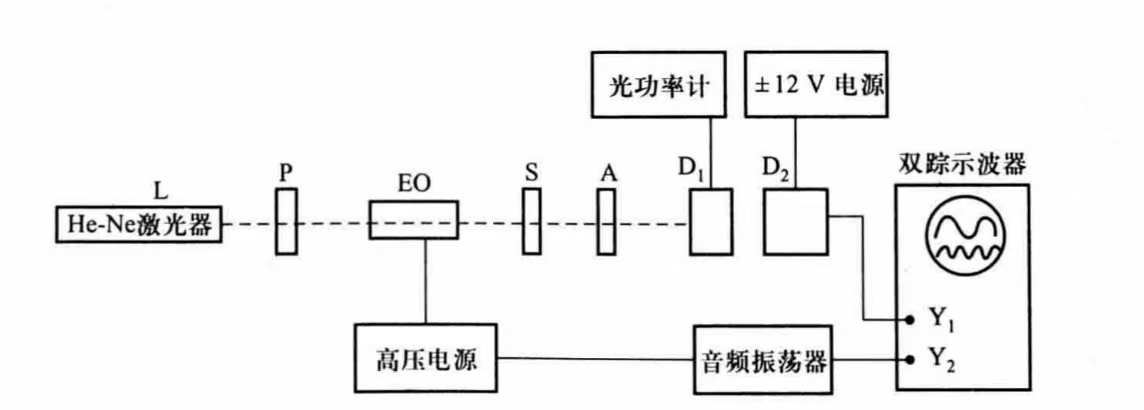
\includegraphics[width=0.85\linewidth]{fig/instrument1.png}
  \label{fig:instrument1}
\end{figure}

图中,光源是He-Ne激光器,输出激光波长为632.8nm,输出功率为5mW

P,A为偏振片,装在带有刻度转盘的支架上

EO为四小块串联的KD*P晶体 

$D_1$为直流光强接受装置,

交流信号选用正弦波形,频率500Hz,振幅10V,其输出的一路作为基频信号输入示波器,另一路与直流电压共同加在电光晶体上

S为待测样品,本实验选用云母片,其厚度为20微米

以上光学元件器件都放置在同一条光学导轨上

首先进行光路调节。在晶体前调节A与P垂直(此时A后光屏无光点);A放在晶体后,在晶体前放镜头纸,白屏放A前,调节晶体位置使得光点处于亮斑中心;
白屏放A后,再调节晶体位置使得光点位于十字暗线中心,十字暗线均分圆。

测零点电压:调节电压直至发现十字中心亮点最暗,此时电压为-180V。
调节过程中可以观察到:当正/负向电压过大时,白屏上出现双曲线,且正负电压时双曲线方向正交

第一次测半波电压:调节电压直至光强功率计示数为极值,此时电压为1440V

第二次测半波电压:调节晶体感应轴与P夹45°,记录光强随着电压的变化。

第三次测半波电压:在晶体上加交流电压,调节晶体上直流电压。
A垂直P时,当$V_{D0}$ = -162V时,输出光极弱,示波器上观测到光强随时间变化频率为2f,此时相位差为0。
A平行P时,当$V_{DP}$ = 1244V时,输出光极弱,示波器上观测到光强随时间变化频率为2f,此时相位差为$\pi$。

测量样品折射率差:将样品两个光轴调节与电光晶体感应轴方向平行,将样品置于晶体与检偏器之间。
当A垂直P,调节V = 338V时输出光极弱。
当A平行P,调节V = 1100V时输出光极弱。



\section{结果及讨论}
通过锥光干涉测得零点漂移电压为-180V

半波电压测量:

法1:$V_{\pi1} = 6480V$

法2:

当A垂直P

\begin{table}[]
\begin{tabular}{llll}
电压(V)                      & 光强(μW)                   & 电压(V) & 光强(μW) \\
-1400                      & 327                      & 100   & 20     \\
-1300                      & 322                      & 200   & 32     \\
-1200                      & 307                      & 300   & 55     \\
-1100                      & 270                      & 400   & 85     \\
-1000                      & 233                      & 500   & 110    \\
-900                       & 197                      & 600   & 160    \\ \cline{1-2}
\multicolumn{1}{|l|}{-800} & \multicolumn{1}{l|}{160} & 700   & 176    \\ \cline{1-2}
-700                       & 120                      & 800   & 210    \\
-600                       & 85                       & 900   & 300    \\
-500                       & 57                       & 1000  & 331    \\
-400                       & 30                       & 1100  & 364    \\
-300                       & 14                       & 1200  & 376    \\
-200                       & 5                        & 1300  & 380    \\
-100                       & 4                        & 1400  & 350    \\
0                          & 8                        &       &       
\end{tabular}
\end{table}

当A平行P

\begin{table}[]
\begin{tabular}{llll}
电压(V)                      & 光强(μW)                   & 电压(V) & 光强(μW) \\
-1400                      & 6                        & 100   & 289    \\
-1300                      & 14                       & 200   & 280    \\
-1200                      & 30                       & 300   & 266    \\
-1100                      & 58                       & 400   & 232    \\
-1000                      & 92                       & 500   & 257    \\
-900                       & 125                      & 600   & 170    \\ \cline{1-2}
\multicolumn{1}{|l|}{-800} & \multicolumn{1}{l|}{150} & 700   & 177    \\ \cline{1-2}
-700                       & 250                      & 800   & 107    \\
-600                       & 270                      & 900   & 80     \\
-500                       & 307                      & 1000  & 47     \\
-400                       & 274                      & 1100  & 22     \\
-300                       & 301                      & 1200  & 6      \\
-200                       & 381                      & 1300  & 4      \\
-100                       & 299                      & 1400  & 13     \\
0                          & 296                      &       &       
\end{tabular}
\end{table}

作图:\autoref{fig:data}

\begin{figure}
  \centering
  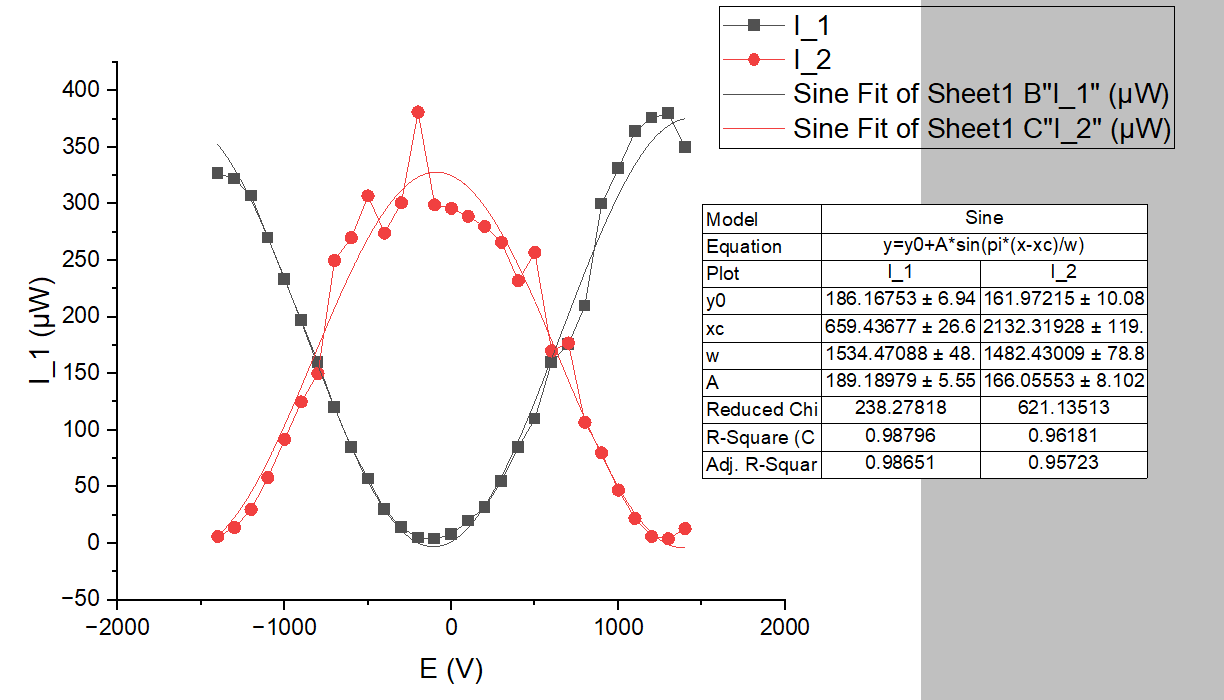
\includegraphics[width=0.8\textwidth]{fig/data.png}
  \label{fig:data}
\end{figure}

通过数据分析并计算后得到半波电压$V_{\pi2} = 6032V$

法3:$V_{\pi3} = 5624V$

根据法2得到的半波电压计算得电光系数$r_{63}$ = 15.3

对样品,根据$V_{\pi2}$及理论中的公式计算得:$\delta n = 0.0035$


\section{结论}
本实验通过三种办法测半波电压得$V_{\pi2} = 6032V$,计算得电光系数$r_{63}$ = 15.3,并测得样品折射率差$\delta n = 0.0035$。
通过这个实验对晶体的电光效应和涉及的相位变化有了更深刻的理解。



\end{document}
